\chapter{Описание разработанных методов}

Для большинства существующих методов решения задачи поиска активного модуля
ответом является некоторый связный подграф заданного графа. Примерами таких
методов являются описанные
ранее~\cite{Ideker2002,Dittrich2008a,Alcaraz2012,Sergushichev2016}.  Общей
проблемой этих методов является необходимость выбора некоторого порога
значимости. При этом, если, например, ослабить такой порог, то размер решения
увеличится за счет добавления новых вершин, но некоторые вершины могут
и пропасть (например, как на рисунке \ref{fig:consistency}). Такое поведение
особенно неудобно с точки зрения пользователя, и усложняет интерпретируемость
результатов.
\begin{figure}
    \begin{subfigure}{.45\textwidth}
        \centering
        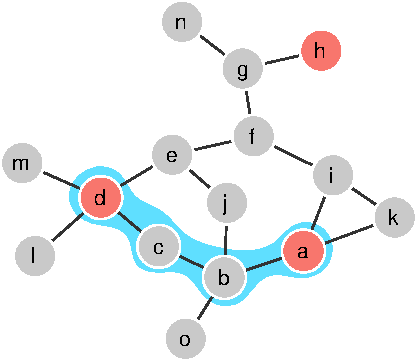
\includegraphics{new-consistency4.pdf}
        \caption{строгий порог\\поиск подграфа размера $4$}
    \end{subfigure} %
    \begin{subfigure}{.45\textwidth}
        \centering
        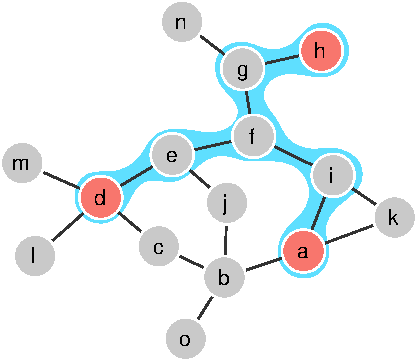
\includegraphics{new-consistency7.pdf}
        \caption{слабый порог\\поиск подграфа размера $7$}
    \end{subfigure}
    \centering
    \caption{
        Вероятно важные вершины и вершины, о которых мало, что известно покрашены
        в красный и серый цвет соответственно.  Синим цветом выделен значимый
        подграф при заданном пороге.  В панелях требуется найти значимый
        подграф заданного размера с максимальным количеством важных вершин.
        Рисунок иллюстрирует несоответствия решений с разными порогами, то есть
        в решение задачи со слабым пороговым значением не входят все вершины из
        решения со строгим пороговым значением.
    }
    \label{fig:consistency}%
\end{figure}

В этом разделе мы рассматриваем формулироваку задачи поиска активного 
модуля в виде сохраняющего связность ранжирования вершин (как на рисунке \ref{fig:rankgraph}).
Такой подход позволяет находить модули для разных порогов, 
совместимые между собой: модуль для более строгого порога
является подмодулем для более слабого порога.
%В разделе~\ref{sec_formal_defs} вводится формальное определение
%задачи. Затем в разделах~\ref{sec_optimal} и~\ref{sec_semiheuristic}
%предлагаются два метода для решения задачи: точный, основанный на
%динамическом программировании по подмножествам, и полуэвристический
%метод, использующий сведение к задаче целочисленного линейного
%программирования. В разделе~\ref{sec_experiments}
%приводится срванение предлагаемых методов с базоывми методами
%на сгенерированных и реальных сетях.





\section{Задача поиска активного модуля в виде ранжирования}
\label{sec_formal_defs}

В этом разделе мы даем формальное определение задачи восстановления активного
модуля в виде ранжирования. Здесь мы рассматриваем только сети с простой
структурой неориентированного графа.

\begin{definition}
    Пусть $G = (V, E)$ граф, тогда \textbf{вершинное ранжирование} графа $G$ есть
    перестановка его вершин $V$.  Для ранжирования $r = (r_1, r_2, \ldots,
    r_{|V|})$ вершины в начале $r$ (например $r_1, r_2, \ldots$) считаются
    более \textbf{важными} и ранжируются выше, чем вершины в конце (например
    $r_{|V|}, r_{|V|-1}, \ldots$).
\end{definition}

\begin{definition}
    Назовем вершинное ранжирование $r$ связного графа $G$ \textbf{монотонно
    связным}, если все подграфы $G_k$, полученные из префикса ранжирования
    $r_{1..k} = (r_1, \ldots, r_k)$, связные для $\forall k \in {1..|V|}$.
\end{definition}

Для удобства рассмотрим префикс ранжирования $r_{1..k}$ как множество $\{r_1, \ldots,
r_k\}$, а не вектор, если этого требует контекст.

В работе используется мера \emph{площади под кривой} (\emph{Area Under Curve},
\emph{AUC}) \emph{рабочая характеристика приёмника} (\emph{Receiver Operating
Characteristic}, \emph{ROC}), чтобы определить, какое ранжирование $r$ графа $G$ лучше
восстанавливает активный модуль $M$.

\begin{definition}
    Значение \emph{AUC ROC} для вершинного ранжирования $r$ графа $G = (V, E)$
    и активного модуля $M \subset V$ считается по формуле:
    \[ AUC~ROC(r \mid M) = \sum_{i=1}^n \left( 1 - \frac{|r_{1..i} \setminus M|}{|V
    \setminus M|} \right) \frac{[r_i \in M]}{|M|}, \]
    где $[r_i \in M]$ индикатор множества $M$.
\end{definition}

Определим рассматриваемую задачу следующим образом.
\begin{problem}[Восстановления активного модуля в виде ранжирования]
    Даны связный граф $G$, неизвестный активный модуль $M$ и веса вершин $w$ из
    бета- и равномерного распределения для вершин из $M$ и $V \setminus M$
    соответственно. Найти монотонно-связное ранжирование $r$ с максимальным
    значением $AUC~ROC(r \mid M)$.
\end{problem}

В дальнейшем будем считать параметр $a$ из бета-распределения $B(a, 1)$
известным. Аналогично~\cite{Dittrich2008a} можно посчитать параметры смеси
бета-равномерного распределения из множества значений функций $\omega$ (весов
вершин) с помощью принципа максимального правдоподобия.

\begin{figure}
    \centering
    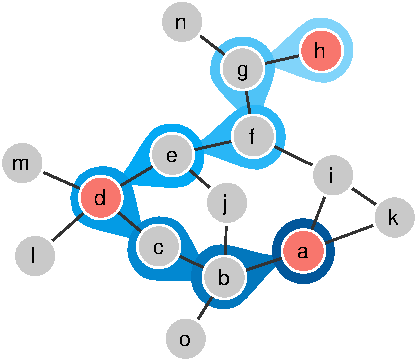
\includegraphics[width=0.5\textwidth]{new-rankgraph.pdf}
    \caption{
        Вероятно важные вершины и вершины, о которых мало что известно, покрашены
        в красный и серый цвет соответственно.  Разными оттенками синего цвета
        проилюстрированы первые семь вершин из монотнно-связного ранжирования.
        Вершины с высоким рангом имеют более темный оттенок синего цвета.
    }%
    \label{fig:rankgraph}%
\end{figure}





\section{Базовые методы}
\label{sec_baseline}

В качестве сравнения для экспериментов рассмотрим следующие два базовых метода.

Первый метод ранжирует вершины по их весам (или по \emph{P}-значениям): чем
меньше вес, тем выше ранг.  Это ранжирование не является монотонно-связным, но
является хорошей отправной точкой.  Этот метод будем называть
\emph{немонотонным} ранжированием.  Заметим, что у этого метода больше степеней
свободы.

Второй метод заключается в использовании алгоритма \emph{BioNet} для десяти
разных пороговых значений.  Поскольку модули BioNet $(M_1, M_2, \ldots,
M_{10})$ могут быть немонотонными, используется следующая процедура
комбинирования.  Присваивается наивысший ранг вершинам из $M_1$, за ними идут
вершины из -- $M_2 \setminus M_1$, после -- $M3 \setminus (M_1 \cup M_2)$
и т.д. Пороговые значения выбираются для распределения на равные отрезки
логарифмических правдоподобий между их максимальными и минимальными значениями.
Этот метод назовем ранжированием на основе \emph{BioNet}.





\section{Оптимальное в среднем ранжирование}
\label{sec_optimal}

В этом разделе мы описываем метод, который находит ранжирование с максимальным
математическим ожиданием \emph{AUC ROC}. Соответственно, мы называем его
методом \emph{оптимального в среднем}.

Во-первых, рассмотрим множество $D \subset 2^V$ всех подмножеств вершин, из
которых получаются связные подграфы графа $G$ и дискретную вероятность $P(M)$,
определенную для всех $M \in D$. Все это вместе составляет вероятностное
пространство $\mathcal{M}$.

Наша задача -- найти ранжирование $r$, максимизирующее математическое ожидание
величины \emph{AUC ROC} для заданных весов вершин $w$:
\begin{equation} \label{formula:eauc} 
    E[AUC~ROC(r \mid \mathcal{M})] = \sum_{M \in D} P(M \mid w) \cdot AUC~ROC(r
    \mid M).
\end{equation}

Условную вероятность модуля $P(M \mid w)$ можно вычислить по теореме Байеса:
\begin{align}
    P(M \mid w) &= \frac{P(w \mid M) \cdot P(M)}{P(w)} = \notag \\
    &= \frac{P(M)}{P(w)} \cdot \prod_{v \in M} B(a,1)(w(v)) \cdot \prod_{v
    \in {V \setminus M}} U(0,1)(w(v)).
\end{align}

Перепишем формулу~\ref{formula:eauc}:
\begin{align}
    E[AUC~ROC(r \mid \mathcal{M})] = \sum_{M \in D} p(M \mid w) \sum_{i=1}^n \left(
    1 - \frac{|r_{1..i} \setminus M)|}{|V \setminus M|}\right) \frac{[r_i \in
      M]}{|M|} = \notag\\
    =  \sum_{i=1}^n \sum_{M \in D}  \left(
    1 - \frac{|r_{1..i}\setminus M|}{|V \setminus M|}\right) \cdot \frac{p(M \mid w)
      \cdot [r_i \in M]}{|M|}.
\end{align}

Это позволит нам посчитать значение $E[AUC~ROC(r \mid \mathcal{M})]$ итеративно:
\begin{multline} \label{eqn:edp}
    E[AUC~ROC(r_{1..k} \mid \mathcal{M})] = E(AUC~ROC(r_{1..k-1} \mid
    \mathcal{M})) + \\ \sum_{M \in D \mid r_k \in M} \left( 1 - \frac{|r_{1..k}
    \setminus M|}{|V \setminus M|}\right) \cdot \frac{p(M \mid w)}{|M|}. 
\end{multline}

Формула \eqref{eqn:edp} позволяет нам посчитать каждый $r_{1..k}$ префикс
ранжирования только один раз.

Это можно использовать, чтобы найти лучшее ранжирование, как показано
в алгоритме~\ref{alg:dp}.  Мы заполняем массив, который для каждого набора
вершин $D[i]$ из $D$ содержит пару значений $dp[i].auc$ -- ожидаемое значение
\emph{AUC ROC} лучшего монотонно-связного ранжирования вершин $D[i]$ и $dp[i].ranking$
-- соответствующее ранжирование. Функция $getArea()$ считает второе слагаемое
формулы~\eqref{eqn:edp}.

\begin{algorithm}
    \caption{Оптимальное в среднем ранжирование.}\label{alg:dp}
    \begin{algorithmic}[1]
        \Procedure{OptimalRanking}{$V$, $E$}
        \State $D \gets getConnectedSubgraphs(V, E)$  \Comment{элементы $D$ сортированы по размеру}
        \State $dp[D]$ : (auc: Double, ranking: Vector)
        \For{$i=1$ to $|D|$}
            \State $M \gets D[i]$
            \ForAll{$v \in M$}
                \If{$isNotConnected(M \setminus \{v\})$}
                    \State \textbf{continue}
                \EndIf
                \State $j \gets$  get index of $M \setminus \{v\}$ in $D$
                \State $auc \gets dp[j].auc + getArea(D, dp[j].ranking, v)$
                \If{$auc > dp[i].auc$}
                    \State $\bar{v} \gets (dp[j].ranking, v)$
                    \State $dp[i] \gets (\bar{v}, auc)$
                \EndIf
            \EndFor
        \EndFor
        \State \textbf{return} $dp[|D|].ranking$
        \EndProcedure
    \end{algorithmic}
\end{algorithm}

Временная сложность алгоритма~\ref{alg:dp} $O(n^2 \cdot |D|^2)$.  Один вызов
функции \emph{getArea()} требует $O(n \cdot |D|)$ времени и это умножается на
$O(n \cdot |D|)$ для внешного цикла. 





\section{Полуэвристическое ранжирование}
\label{sec_semiheuristic}

В этом разделе описывается еще один подход к решению задачи ранжирования
вершин.  Этот подход основан на методе \emph{BioNet}~\cite{Dittrich2008a}
и заключается в решении серии задач \emph{целочисленного линейного
программирования} (\emph{Integer Linear Programming}, \emph{ILP}). По сравнению
с подходом оптимального в среднем из предыдущего раздела, этот метод позволяет
найти ранжирование для больших графов за довольно разумное время.  Поскольку
метод явно не оптимизирует оценку \emph{AUC ROC}, мы называем его
\emph{полуэвристическим} (рисунок~\ref{fig:shranking}).
\begin{figure}
    \begin{subfigure}{.5\textwidth}
        \centering
        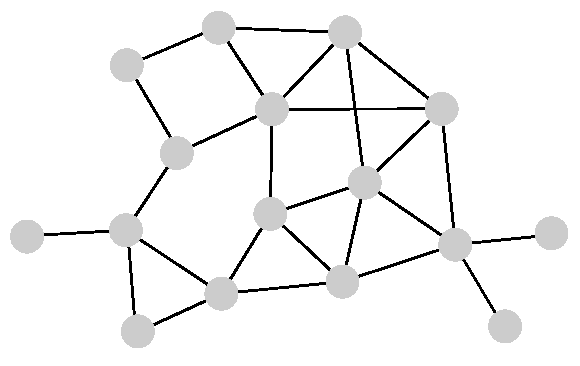
\includegraphics[width=\textwidth]{shmyak-illustration1}
        \caption{Исходный граф} 
    \end{subfigure}%
    \begin{subfigure}{.5\textwidth}
        \centering
        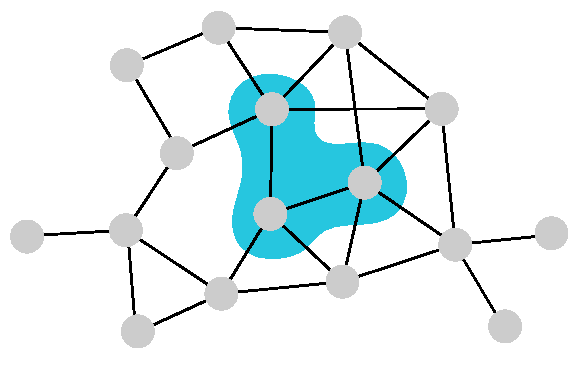
\includegraphics[width=\textwidth]{shmyak-illustration2}
        \caption{Найденный активный модуль}
    \end{subfigure}\\[1ex]
    \begin{subfigure}{.5\textwidth}
        \centering
        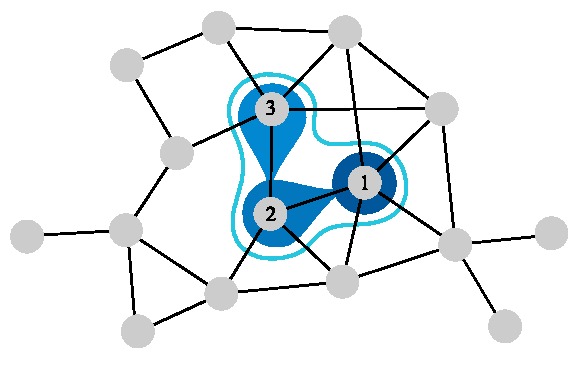
\includegraphics[width=\textwidth]{shmyak-illustration3}
        \caption{Ранжирование внутри модуля}
    \end{subfigure}%
    \begin{subfigure}{.5\textwidth}
        \centering
        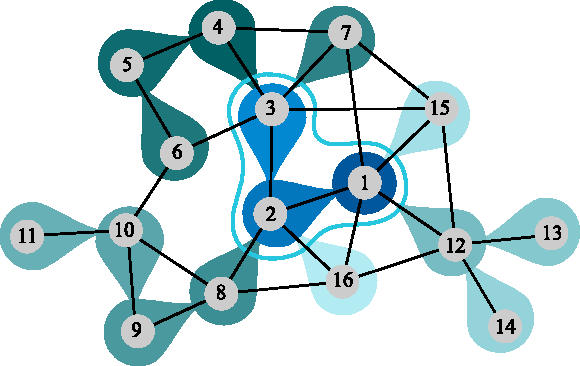
\includegraphics[width=\textwidth]{shmyak-illustration4}
        \caption{Ранжирование оставшихся вершин}
    \end{subfigure}
    \centering
    \caption{
        Иллюстрирует этапы полуэвристического метода.  В панели (a) дается
        связный взвешанный граф.  В панели (b) красным цветом отмечен \emph{MWCS}.
        В панели (c) рекурсивно запускается полуэвристический алгоритм
        и ранжируются все его вершины.  В панели (d) ранжируются серые
        (оставшиеся) вершины.
    }%
    \label{fig:shranking}%
\end{figure}
Сначала, подобно \emph{BioNet}, найдем подграф $G$, который скорее всего будет
активным модулем.  Наиболее вероятный подграф имеет наилучшую оценку
логарифмического правдоподобия.  Оценка логарифмического правдоподобия модуля
может быть рассчитана как сумма оценок логарифмического правдоподобия отдельных
вершин в модуле, где индивидуальная оценка для вершины $v$ вычисляется как: \[
    score(v) = \log \mathcal{L} (a, 1 \mid w(v)) = \log(a \cdot {w(v)}^{a - 1}).\]

Теперь мы можем найти связный подграф $M$ с максимальной суммой оценок вершин.
Это соответствует экземпляру задачи \emph{MWCS}. Эта задача является
\emph{NP}-трудной, но ее можно свести к задаче \emph{ILP} и воспользоваться его
решателем для решения нашей задачи.

Используя найденный подграф $M$, определяется грубое частичное ранжирование,
сказав, что вершины $M$ идут до $V \setminus M$.

Затем мы определяем процедуру для уточнения такого частичного ранжирования.
Эта процедура принимает два набора вершин: множество $R$, содержащее уже
ранжированные вершины, и множество $C$, содержащее множество кандидатов,
которые должны быть ранжированы. Тогда найдем подмножество $X$ из $C$, такое
что $R \cup X$ связано, и вершины из $X$ должны быть ранжированы выше, чем
вершины из $C \setminus X$.

Используя эту процедуру, мы можем рекурсивно уточнить ранжирование до уровня
отдельных вершин. На этапе инициализации $R$ задается пустым множеством, а $C$
содержит все вершины.  Затем выполняется ранжирование для $(R, X)$ и $(R \cup
X, C \setminus X)$.  Мы останавливаем рекурсию, когда набор кандидатов состоит
только из одной вершины.

Параметр этой процедуры состоит в том, как выбрать набор $X$.  Для этого,
аналогично первому шагу, мы решаем задачу \emph{MWCS}, но с дополнительным
ограничением, которое требует, чтобы решение содержало по крайней мере одну
вершину из $R$ и по меньшей мере одну, но не все вершины из $C$. Положим $X$
как пересечение решения и множества $C$.  Соответствующая задача решается
модифицированным решателем из~\cite{Loboda2016}, где соответствующие
ограничения были добавлены в формулировку \emph{ILP}.

Общий алгоритм приведен в алгоритме~\ref{alg:shmyak}.  Процедура
\emph{findMaximumSG()} решает \emph{MWCS} с описанными дополнительными
ограничениями и возвращает выбранное подмножество вершин из $C$.  Если размер
$list$ больше одного, мы вызываем \emph{refineRanking()}, чтобы получить
ранжирование этого множества. Алгоритм возвращает ранжирование $r$ вершин
множества $C$.  Пример выполнения алгоритма приведен на
рисунке~\ref{fig:shexample}.

\begin{algorithm}[h!]
    \caption{Обработка полуэвристического ранжирования.}\label{alg:shmyak}
    \begin{algorithmic}[1]
        \Procedure{RefineRanking}{ $V$, $E$, $R$, $C$}
        \State $r$ : Ranking
        \While{$C.size \not= 0$}
            \State $list \gets  findMaximumSG(V, E, R, C)$
            \If{$list.size > 1$}
                \State $list \gets refineRanking(V, E, R, list)$
            \EndIf
            \State $r.addAll(list)$
            \State $R.addAll(list)$
            \State $C.removeAll(list)$
        \EndWhile
        \State \textbf{return} $r$
        \EndProcedure
    \end{algorithmic}
\end{algorithm}

\begin{figure}
    \begin{subfigure}{.5\textwidth}
        \centering
        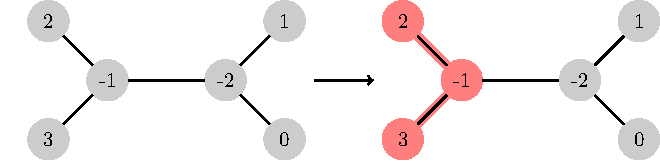
\includegraphics[width=1.0\textwidth]{shexample1.pdf}
        \caption{\footnotesize{Исходный граф и подграф максимального веса}} 
    \end{subfigure}%
    \begin{subfigure}{.5\textwidth}
        \centering
        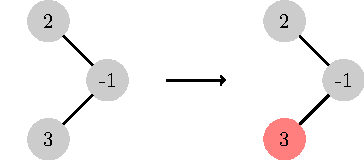
\includegraphics[width=.55\textwidth]{shexample2.pdf}
        \caption{\footnotesize{Ранжирование связного подграфа}}
    \end{subfigure}\\%[1ex]
    \begin{subfigure}{.5\textwidth}\centering
        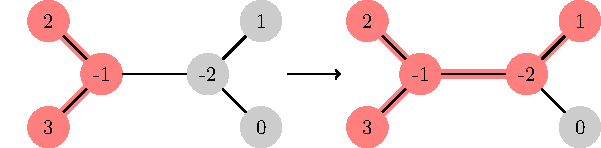
\includegraphics[width=1.0\textwidth]{shexample3.pdf}
        \caption{\footnotesize{Ранжирование оставшихся вершин}}
    \end{subfigure}%
    \begin{subfigure}{.5\textwidth}
        \centering
        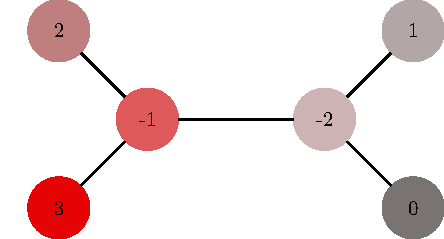
\includegraphics[width=.45\textwidth]{shexample4.pdf}
        \caption{\footnotesize{Финальное ранжирование}}
    \end{subfigure}
    \centering
    \caption{
        Пример работы полуэвристического метода.  В панели (a) из исходного
        графа находим связный подграф максимального веса (отмечен красным
        цветом).  Далее в панели (b) ранжируются веса вершин связного подграфа
        с помощью запуска в нем рекурсивного полуэвристического метода.
        В панели (c) приводится этап ранжирования оставшихся вершин.  На выходе
        мы получаем ранжирования в панели (d), где вершины более красного
        оттенка идут раньше остальных вершин.
    }%
    \label{fig:shexample}%
\end{figure}





\section{Задача оценки вероятности принадлежности вершины к модулю}
%TODO: переписать всю 

% В то время как задача поиска активного модуля проявляется во многих разных
% контекстах, для ясности мы фокусируемся здесь на примере сети белок-белковых
% взаимодействий вместе с данными экспрессии генов.  Мы формализуем сеть
% белок-белковых взаимодействий как граф $G$, где вершины соответствуют
% белок-кодирующим генам, и две вершины связаны ребром, если взаимодействуют
% соответствующие белки.  Данные экспрессии гена приведены для набора образцов
% для двух представляющих интерес биологических условий (например, контрольная
% и лечения), так что $P$-значения дифференциального экспрессия  могут быть
% вычислены для каждого гена.  Хотя для некоторых генов нулевая гипотеза верна,
% и поэтому соответствующие $P$-значения равномерно распределены на отрезке $[0,
% 1]$, $P$-значения для «интересных» генов, которые имеют разницу в экспрессии,
% имеют тенденцию быть ближе к нулю.  Согласно~\cite{Ideker2002}, эти <<интересные>>
% гены образуют связный подграф в $G$, который называется активным (или
% функциональным) модулем.

Как показано в~\cite{Pounds2003,Dittrich2008a}, распределение всех $P$-значений
может быть аппроксимировано с помощью смеси \emph{BUM} распределения, где бета
составляющая соответствует сигналу в данных, а равномерная составляющая
соответствует шуму.  Напомним, что бета-распределение имеет носитель на $[0,
1]$ и определяется его плотностью:
\[\beta(a,b)(x) = \frac{1}{B(a,b)} x^{a-1}(1-x)^{b-1},\]
где $B(a, b)$ -- бета-функция. Распределение BUM представляет собой смесь
равномерного и бета $\beta(a, 1)$ распределений и определяется его плотностью:
\[\lambda +(1-\lambda)\beta(a,1)(x),\]
где $\lambda$ -- доля смеси равномерной составляющей, $a$ -- параметр
бета-распределения.

Мы присваиваем вес $w(v)$ каждой вершине $v$ графа $G$, равному $P$-значению,
присвоенному соответствующему гену.  Таким образом, в нашей модели мы имеем:
связный граф $G$, его связный подграф $M$, семейство независимых случайных
величин $W_v$, $v \in V (G) \setminus V(M)$ с равномерным распределением на
$[0, 1]$ и семейство независимых случайных величин $W_v$, $v \in V (M)$
с распределением $\beta(a, 1)$.

%TODO: Написать где-то про пространства весов
Наша цель - выяснить, какие вершины принадлежат активному модулю $M$:
\begin{problem}[Оценка вероятности принадлежности активному модулю]
    Дан связный граф $G$ и веса вершин $w_v \in \mathbb{R}$, найти вероятность
    $P(v \in M \mid W = w)$ принадлежности каждой вершины $v$ к модулю $M$.
    \label{pr:probability}
\end{problem}

Параметры \emph{BUM} распределения $а$ и $\lambda = 1 - \frac{|M|}{|V|}$
можно оценить с помощью максимального правдоподобия~\cite{Beisser2010}.
Мы предпологаем, что $a$ и $|M|$ известны.





\section{Метод, основанный на методе Монте-Карло по схеме марковских цепей}

В этом разделе мы предлагаем метод оценивания вероятности принадлежности вершин
к активному модулю, то есть решения задачи \ref{pr:probability}.  Метод основан
на методе Монте-Карло по схеме марковских цепей (\emph{Markov Chain Monte
Carlo}, \emph{MCMC}).

Решаем задачу \ref{pr:probability} следующим образом: выбирается множество
$\mathbb{S}$ случайных подграфов $S$ из условного распределения $P(S = M \mid
W = w)$ с использованием подхода \emph{MCMC} и оценим $P(v \in M|W = w)$ как:
\[P(v \in M \mid W = w) \approx \frac{|\{S \in \mathbb{S} : v \in
S\}|}{|\mathbb{S}|} \, .\]

Для выборки c использованием \emph{MCMC} мы применяем алгоритм
Метрополиса-Гастингса~\cite{Hastings1970}.  Он начинает со случайного подграфа
$S_0$ размера $k=|M|$. На каждом шаге $i$ мы выбираем подграф кандидата $S'$
путем удаления вершины $v_-$ из $S_i$ и добавления другой вершины $v_+$ из
окрестности $S_i$ (под окрестностью подграфа $S:$
\[\operatorname{nei}(S) = \{v \in G: \min_{u \in S} dist(v,u) =1\}\]
мы имеем в виду множество всех вершин из $G$ на расстоянии $1$ от $S$).
Заметим, что подграф $S'$ всегда имеет такое же число вершин $k$, что и $S_0$.
Вспомогательная функция распределения $Q(S' \mid S_i)$ равна
\[Q(S' \mid S_i) = \frac{1}{|\operatorname{nei}(S_{i})| \cdot |V(S_i)|} \, .\]

Мы установили вероятность принятия в алгоритме Метрополиса-Гастингса как:
\[\rho(S_i,S') = \min \left\{1,\frac{P(S'=M \mid W = w)}{P(S_i=M \mid
W = w)}\frac{Q(S_i \mid S')}{Q(S' \mid S_i)} \right\} \, ,\]
где $P(S'=M \mid W = w) = 0$, если $S'$ становится несвязным. 

Для любого связного подграфа $S$ графа $G$, значение $P(S=M \mid W=w)$ может
быть выражено через плотность вероятности $p$ абсолютно непрерывной случайной
векторной переменной $W$:
\begin{align}
    P(S=M \mid W = w) = \frac{p(w \mid S=M)P(S=M)}{p(w)} \, .
    \label{eq:graphprobs}
\end{align}
Таким образом,
\[\frac{P(S'=M \mid W = w)}{P(S_i=M \mid W = w)} = \frac{p(w \mid
S'=M)P(S'=M)}{p(w)}\frac{p(w)}{p(w \mid S_i=M)P(S_i=M)} \, .\]
Дробь $\frac{p(w \mid S'=M)}{p(w \mid S_i=M)}$ равна
\begin{align}
    \frac{p(w \mid S'=M)}{p(w \mid S_i=M)} = \frac{L(S')}{L(S_i)} \, ,
    \label{eq:likelihood}
\end{align}
где $L(S)$ -- правдоподобия подграфа $S$. В нашем случае
\[L(S) = \prod_{v\in S}\beta(a,1)(w_v) \, ,\]
так, мы имеем:
\begin{align}
    \frac{p(w \mid S'=M)}{p(w \mid S_i=M)} = \frac{\prod_{v\in S'}\beta(a,1)(w_v)}{\prod_{u\in S_i}\beta(a,1)(w_u)} = \frac{\beta(a,1)(w_{v_+})}{\beta(a,1)(w_{v_-})} \, .
    \label{eq:accept_probs}
\end{align}

Предполагая, что априорное распределение выбора модуля $P(S=M)$
равномерно\footnote{Поскольку мы не делаем никаких дополнительных предположений
о модуле, равномерное распределение на подграфах равного размера является
наилучшим выбором априорного распределения.} на множестве связных подграфов $S$
такого же размера $|M|$, получаем
\[ \rho(S_i,S') = \min \left\{1,
\frac{\beta(a,1)(w_{v_+})}{\beta(a,1)(w_{v_-})}
\frac{|\operatorname{nei}(S_{i})|}{|\operatorname{nei}(S')|} \right\} \, .\]

Алгоритм Метрополиса-Гастингса с вышеперечисланными параметрами может посещать
все возможные подграфы $S$, и поэтому он сходится к распределению $P(S=M|W=w)$.
На рисунке~\ref{recombiter} показаны этапы итераций.

\begin{algorithm}
    \caption{Алгоритм Метрополиса-Гастингса}
    \label{alg:mh}
    \begin{algorithmic}[1]
        \State Инициализируем $S_0$ как случайный связный подграф из $k=|M|$ вершин\;
        \For{$i = 0,1,2,\dots$}
            \State Выберем $v_-$ из $S_i$ и $v_+$ из $nei(S_i)$ равномерно\;
            \State Порожденный подграф $S'$ из вершин $S_i \setminus\{v_-\}\cup \{v_+\}$\;
            \If{$S'$ \emph{связный}}
                \State Вероятность принятия:
                $\rho(S_i,S') = \min \left\{1, \frac{\beta(a,1)(w_{v_+})}{\beta(a,1)(w_{v_-})} \frac{|\operatorname{nei}(S_{i})|}{|\operatorname{nei}(S')|} \right\}$\;
                \State $S_{i+1} := 
                    \begin{cases}
                        S' \emph{ с вероятностью } \rho(S_i,S')\\
                        S_i \emph{ с вероятностью }  1-\rho(S_i,S')\\
                    \end{cases}$
            \Else
                \State $S_{i+1} := S_i\;$
            \EndIf
        \EndFor
    \end{algorithmic}
\end{algorithm}

\begin{figure}
    \begin{subfigure}{.5\textwidth}
        \centering
        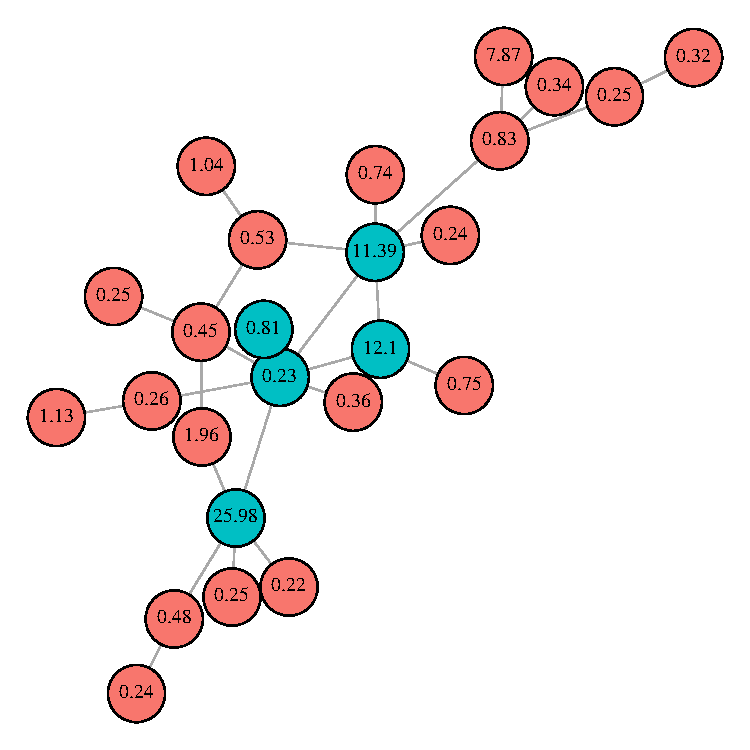
\includegraphics[width=.75\textwidth]{iter1.pdf}
        \caption{Исходный граф и активный модуль} 
    \end{subfigure}%
    \begin{subfigure}{.5\textwidth}
        \centering
        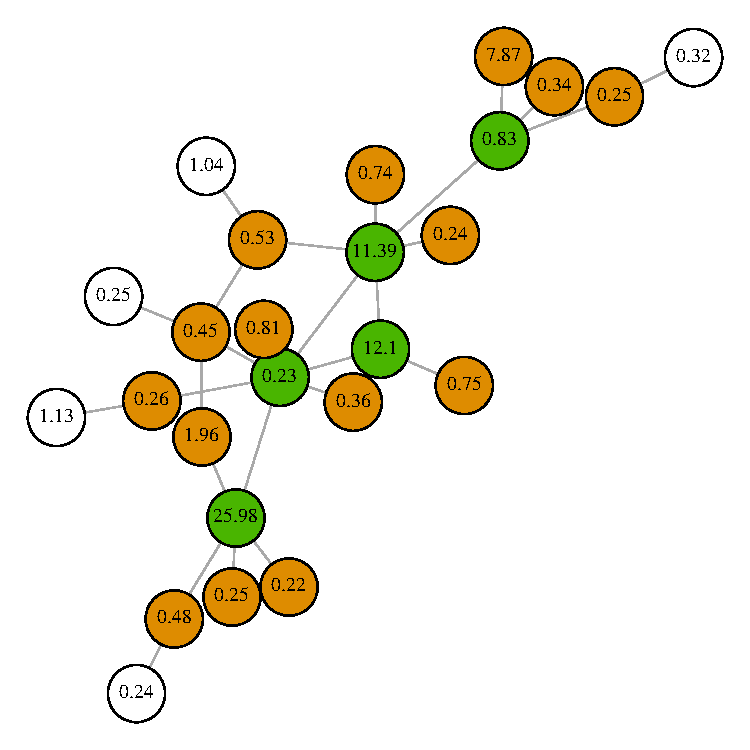
\includegraphics[width=.75\textwidth]{iter2.pdf}
        \caption{Подграфа после $500$ итераций \emph{MCMC}}
    \end{subfigure}\\[1ex]
    \begin{subfigure}{.5\textwidth}
        \centering
        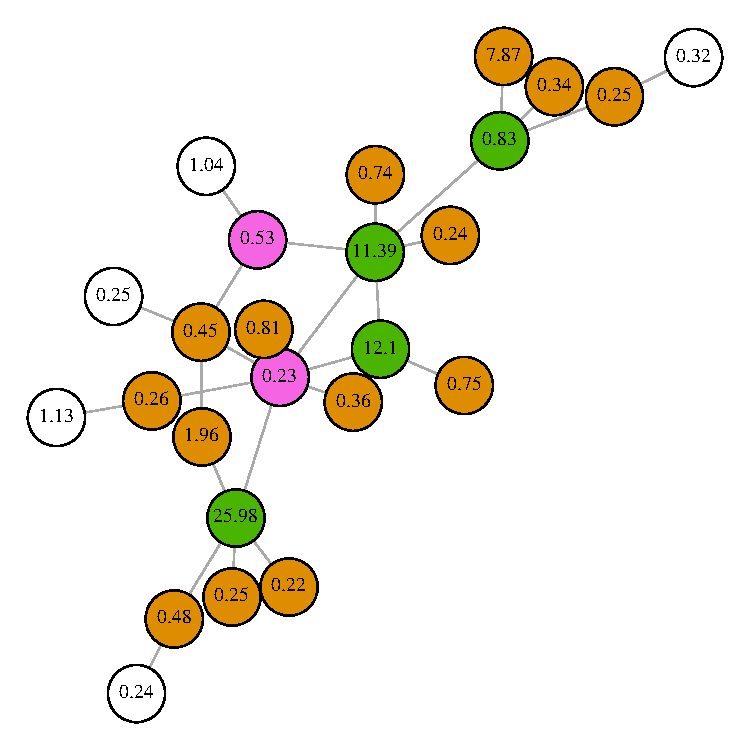
\includegraphics[width=.75\textwidth]{iter3.pdf}
        \caption{Подграф становится несвязным}
    \end{subfigure}%
    \begin{subfigure}{.5\textwidth}
        \centering
        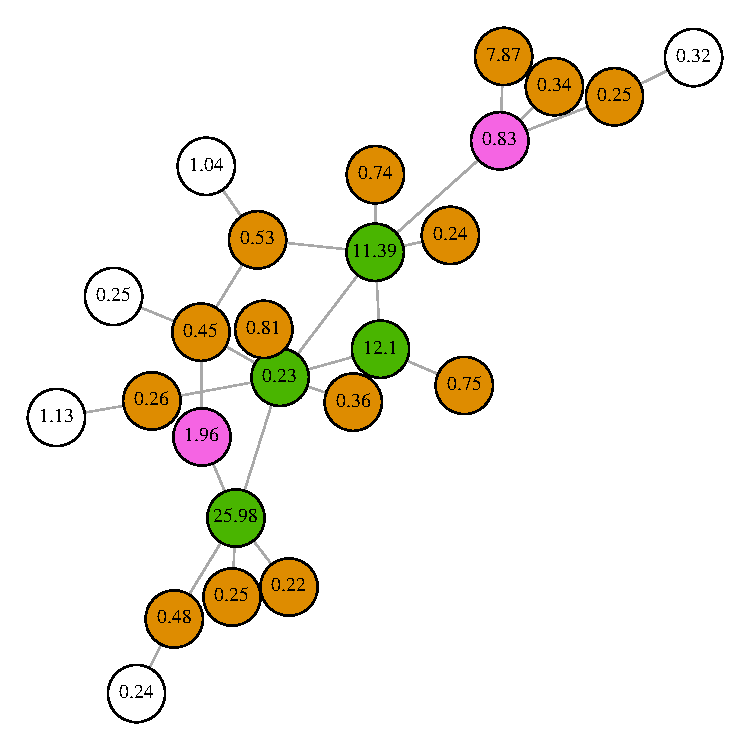
\includegraphics[width=.75\textwidth]{iter4.pdf}
        \caption{Новая итерация, новый кандидат}
   \end{subfigure}\\[1ex]
   \begin{subfigure}{.5\textwidth}
        \centering
        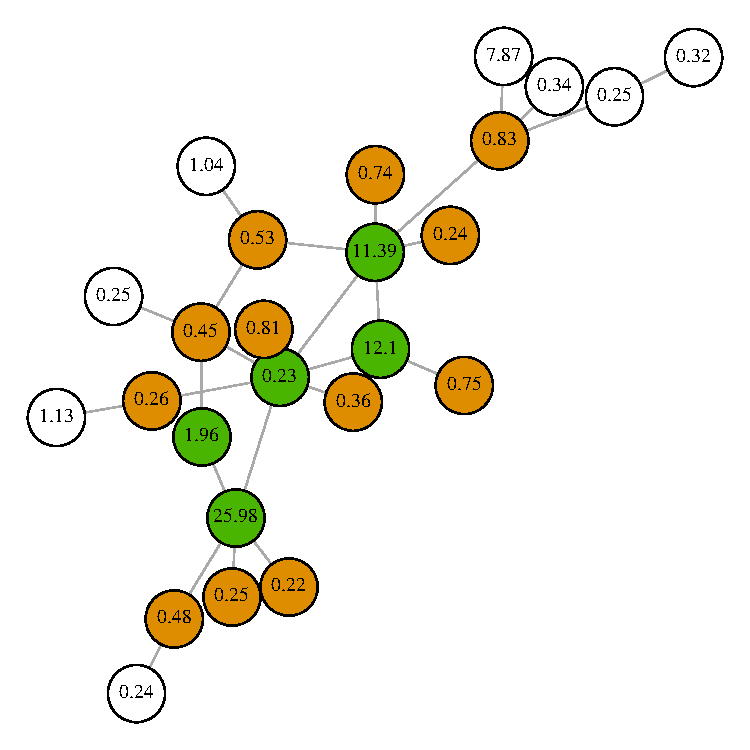
\includegraphics[width=.75\textwidth]{iter5.pdf}
        \caption{Успешное принятие кандидата} 
   \end{subfigure}%
   \begin{subfigure}{.5\textwidth}
        \centering
        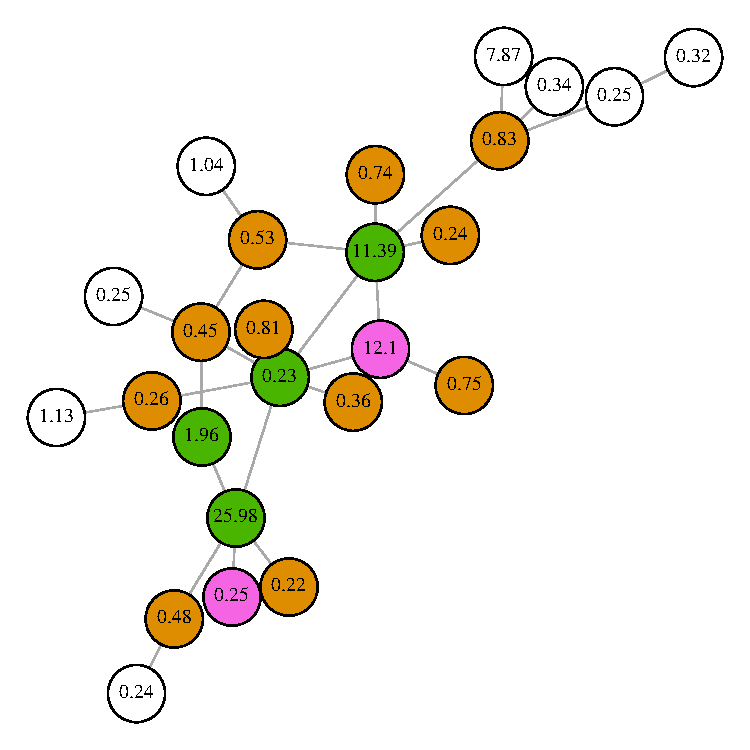
\includegraphics[width=.75\textwidth]{iter6.pdf}
        \caption{Итерация успешна с вероятностью $\rho=0.02$}
   \end{subfigure}\\[1ex]
    \centering
    \caption{
        Иллюстрация выполнения итераций метода \emph{MCMC}.  Надпись на вершинах
        означает правдоподобие вершин.  В панели (a) вершины из модуля окрашены
        синим цветом, а все остальные красным цветом.  В панелях (b) - (f)
        вершины подграфа и его соседние вершины окрашены зеленым и коричневым
        цветом соответственно. Фиолетовым цветом окрашены вершины изменившие свое
        состояние в этой итерации.
    }%
    \label{recombiter}%
\end{figure}

Для оценки вероятностей $P(v \in M \mid W=w)$ нам нужно выбрать набор образцов
подграфов $\mathbb{S}$.  Здесь мы рассмотрим два способа сделать это.  В обоих
направлениях нам необходимо оценить время $T$ смешивания алгоритма: число
итераций цепи Маркова, так что распределение $S_T$ хорошо аппроксимирует
целевое распределение.  Это время зависит от множества параметров, включая
размер графа $G$.  Первый способ выбора $\mathbb{S}$ состоит в том, чтобы
выполнить ряд независимых \emph{MCMC}-прогонов $T$-итераций и добавить каждый
$S_T$ в $\mathbb{S}$.  Здесь вся выборка в $\mathbb{S}$ независима, что может
быть использовано для вычисления точной оценки вероятностей вершин.  Другой
способ состоит в том, чтобы запустить \emph{MCMC} один раз на длительный период
и положить все $S_i$ для $i>T$ в $\mathbb{S}$.  Хотя последовательные выборки
не являются независимыми, оцененные таким образом вероятности сходятся
к истинной вероятности для достаточно длинного периода запуска.





\section{Оптимизация \emph{AUC ROC}}
В этом разделе рассматривается вопрос как вероятность принадлежности вершин
активному модулю относится к средней кривой \emph{ROC} для некоторого
вершинного ранжирования.  А именно докажем следующую лемму:
\begin{lemma}
\label{lem:auc}
Пусть $n$ -- число вершин в $G$, $m$ -- число вершин в модуле $M$,
$r_1, r_2, \dots, r_n$ - некоторое ранжирование вершин, а $p_i$ - вероятности
$p_i = P (r_i \in M \mid W = w)$.  Тогда среднее значение \emph{AUC ROC} равно
\begin{align*}
    1 - \frac{\sum_{i=1}^{n} i p_i - \frac{m(m+1)}{2}}{m(n-m)}.
\end{align*}
\end{lemma}
\begin{proof}
    Для доказательства мы воспользуемся графиком ненормализованной
    \emph{ROC}-кривой, повернутой на $\frac{\pi}{4}$ (как на рисунке
    \ref{fig:lemma}~(\subref{fig:lemma:roc-rotation})).  Рисунок
    \ref{fig:lemma}~(\subref{fig:lemma:roc-unnorm}) без нормализации
    \emph{ROC}-кривой получен из рисунка
    \ref{fig:lemma}~(\subref{fig:lemma:roc-start}) с помошью растягивания оси
    $x$ и $y$ в $m$ и $n-m$ раз.
    \begin{figure}
            \begin{subfigure}{.5\textwidth}
                \centering
            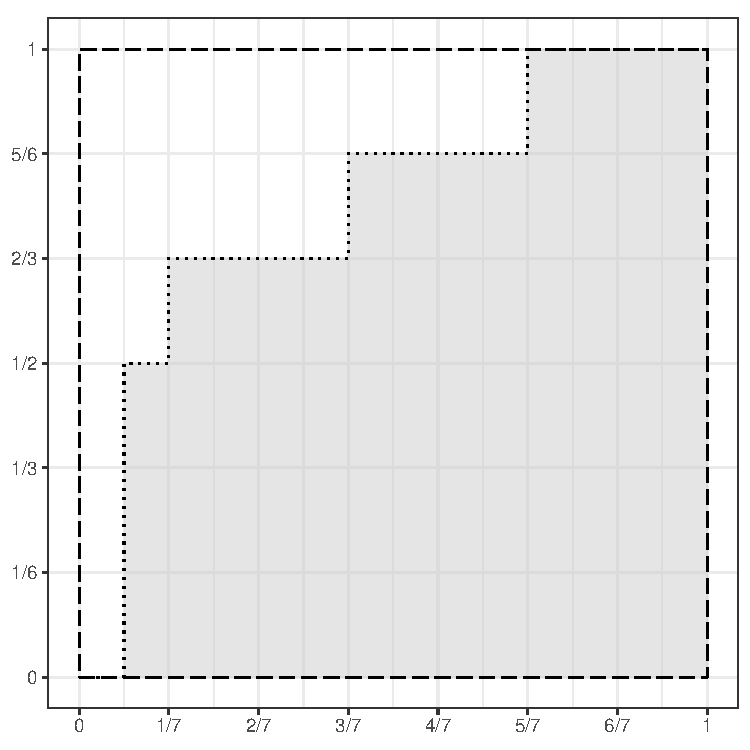
\includegraphics[width=0.95\textwidth]{titanic-roc-01.pdf}
                \caption{График \emph{ROC} кривой} 
            \label{fig:lemma:roc-start}
        \end{subfigure}%
        \begin{subfigure}{.5\textwidth}
            \centering
            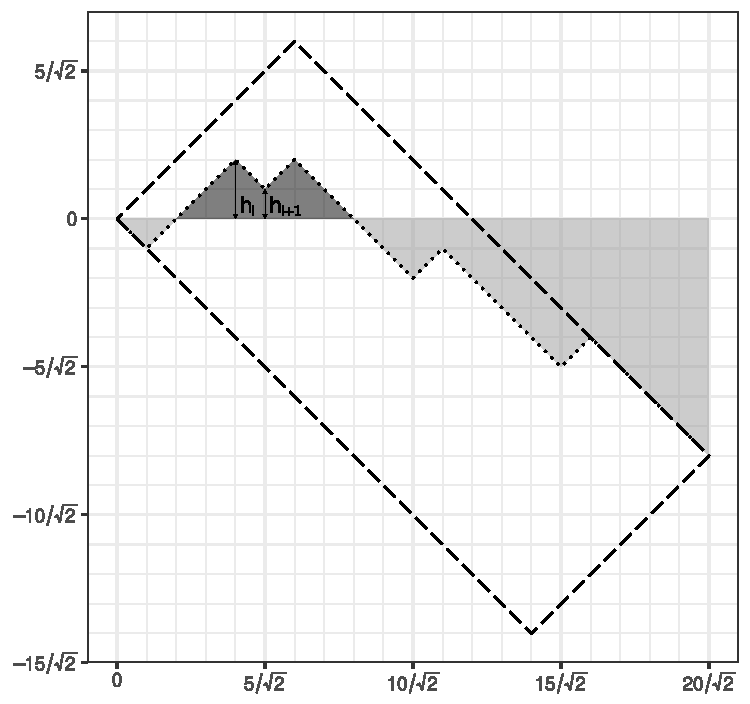
\includegraphics[width=\textwidth]{titanic-roc-final.pdf}
            \caption{\emph{ROC} кривая, повернутая на $\frac{\pi}{4}$}
            \label{fig:lemma:roc-rotation}
        \end{subfigure}\\
        \begin{subfigure}{.5\textwidth}
            \centering
            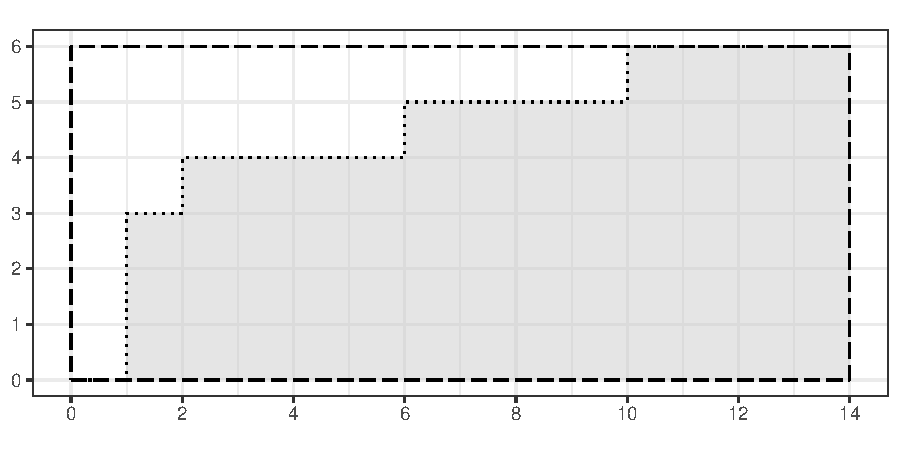
\includegraphics[width=\textwidth]{titanic-roc-02.pdf}
            \caption{\emph{ROC} кривая без нормализации}
            \label{fig:lemma:roc-unnorm}
        \end{subfigure}%
        \begin{subfigure}{.5\textwidth}
            \centering
            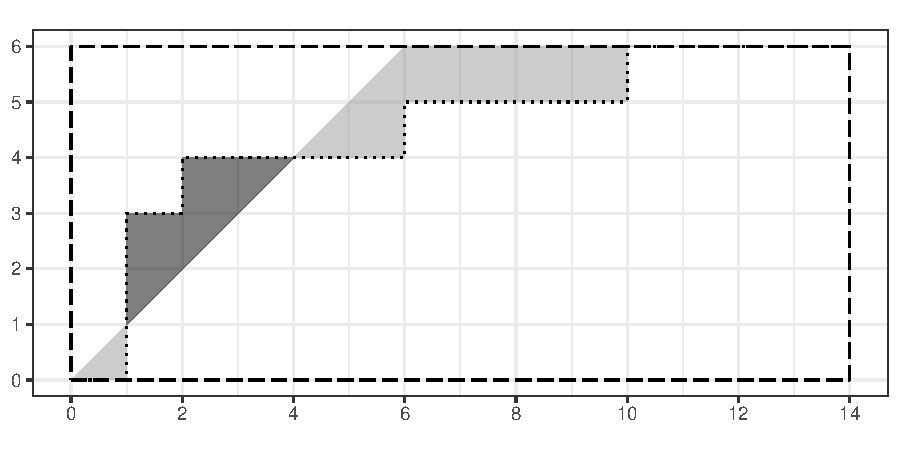
\includegraphics[width=\textwidth]{titanic-roc-03.pdf}
            \caption{\emph{ROC} кривая и прямая $y=x$}
            \label{fig:lemma:roc-idfunc}
        \end{subfigure}
        \centering
        \caption{}
        \label{fig:lemma}%
    \end{figure}

    Пусть $h_i$ -- это средняя высота первых $i$ рангов.  Так как $h_{i-1}$
    с вероятностью $p_i$ и $1-p_i$ поднимается на $\frac{1}{\sqrt{2}}$
    и $-\frac{1}{\sqrt{2}}$ единицу соответственно, то в среднем $h_{i}
    = h_{i-1} + \frac{2p_i-1}{\sqrt{2}}$ (где $h_0=0$).

    Заметим, что сумма вероятностей всех вершин равен значению $m.$

    Плошадь под ненормализованной \emph{ROC}-кривой  повернутой на
    $\frac{\pi}{4}$ считается как сумма пятиугольника и окрашенной области.
    \begin{align*}
        \tilde{E}[AUC ROC(r \mid M)] &=\\
        &= m(n-m) - \frac{m^2}{2}+\frac{(n-2m)^2}{4} + 
            \sum_{i=1}^{n} \frac{h_{i-1}+h_{i}}{2}\frac{1}{\sqrt{2}} = \\
        &= \frac{n^2}{4} - \frac{m^2}{2} +
            \sum_{i=1}^{n} \frac{h_i}{\sqrt{2}} + \frac{h_0 - h_n}{2\sqrt{2}} = \\
        &= \frac{n^2}{4} - \frac{m^2}{2} +
            \sum_{i=1}^{n} \frac{(n+1-i)\frac{2p_i-1}{\sqrt{2}}}{\sqrt{2}} - \frac{\sum_{i=1}^{n} \frac{2p_i-1}{\sqrt{2}}}{2\sqrt{2}} = \\
        &= \frac{n^2}{4} - \frac{m^2}{2} +
            \sum_{i=1}^{n} \frac{(n+1-i)(2p_i-1)}{2} - \frac{\sum_{i=1}^{n} 2p_i-1}{4} = \\
        &= \frac{n^2}{4} - \frac{m^2}{2} +
            \sum_{i=1}^{n} \bigg((n+1)p_i - \frac{n+1-i}{2} -ip_i\bigg)- \frac{2m-n}{4} = \\
        &= \frac{n^2}{4} - \frac{m^2}{2} +
            (n+1)m - \frac{n(n+1)}{4} - \sum_{i=1}^{n}ip_i -\frac{2m-n}{4} = \\
        &= \frac{n^2}{4} - \frac{m^2}{2} +
            nm + m - \frac{n^2}{4} - \frac{n}{4} - \sum_{i=1}^{n}ip_i -\frac{m}{2} + \frac{n}{4} = \\
        &=  - \frac{m^2}{2} +
            nm + \frac{m}{2} - \sum_{i=1}^{n}ip_i = \\
        &=  m(n-m) + \frac{m(m+1)}{2} - \sum_{i=1}^{n}ip_i.
    \end{align*}
    Введя нормализацию получим то, что требовалось доказать.
    \[E[AUC ROC(r \mid M)] = 1 - \frac{\sum_{i=1}^{n}ip_i - \frac{m(m+1)}{2}}{m(n-m)}.\]
\end{proof}

Из леммы \ref{lem:auc} следует, что ранжирование вершин с наибольшим средним
значением \emph{AUC ROC} является ранжирование с убывающим порядком
вероятностей $p_i$ (для любого конкретного размера модуля $m$).





\section{\emph{MCMC} ранжирование}
Предлагается следующий эвристический метод ранжирования по вероятностям
вхождения вершины в активный модуль. Назовем мы его \emph{MCMC} ранжированием.

На этапе инициализации имеются все вершины, которые мы будем итеративно
ранжировать.  Каждая итерация состоит из выбора вершины после удаления которой
средняя вероятность вершин самой большой компоненты связности максимальна.
Выбранная вершина и все вершины из небольшой компоненты связности после
удаления этой вершины получат одинаковый ранг, выше чем у ранее отранжированных
вершин, и удаляются из графа.  Если вместе с выбранной вершиной удаляется
вершина с вероятностью ниже чем у этой вершины, то его кандидатура не
рассматривается. Таким образом, мы итеративно составляем ранжирования (см.
Алгоритм \ref{alg:mcmc}).

\begin{algorithm}
    \caption{Алгоритм \emph{MCMC} ранжирования}
    \label{alg:mcmc}
    \hspace*{\algorithmicindent} \textbf{Input:}  Граф $G=(V, E)$ и веса $p_v$ на вершинах\\
    \hspace*{\algorithmicindent} \textbf{Output:} Монотонно связное ранжирование $r$
    \begin{algorithmic}[1]
        \State Инициализируем ранжирование $r$ пустым;
        \While{$|r| \not= |M|$}
            \State Инициализируем пустое множество вершин $C,$ средняя вероятность $p_{mean}:=1\;$
            \For{$v \in V$}
                \State Выберем большую компоненту связности $C'$ после удаления $v\;$
                \State Вычисляем среднюю вероятность вершин $p'_{mean}$ в $C'\;$
                \State Найдем самую худшую вероятность $p_{min}$ в $C\;$
                \If{$p_v \le p_{min}$ и $p'_{mean} < p_{mean}$}
                    \State $p_{mean} := p'_{mean}\;$
                    \State $C := C'\;$
                    \State $v_x := v\;$
                \EndIf
            \EndFor
            \State $r := (V \setminus C,~r)\;$
            \State $V := C\;$
        \EndWhile
    \end{algorithmic}
\end{algorithm}

Время выбора вершины в каждой итерации составляет $O(n^2)$.  В самом худшем
случае совершается $n$ итераций, и итого весь метод ранжирования работает за
$O(n^3)$.

\chapterconclusion
Жесткая классификация вершин на принадлежность активному модулю при разных
пороговых значениях не согласована и соответственна склонны к плохой
интерпретации.  Поставлена задача ранжирования вершин графа и критерия оценки
ранжирований. Предложены три метода ранжирования вершин.  Поставлена задача
оценки вероятности принадлежности вершин активному модулю и предложен метод
решения этой задачи.
